% !TEX program = xelatex
\documentclass[aspectratio=169]{beamer}
\usepackage{ctex, hyperref}
\usepackage[T1]{fontenc}
\usepackage{latexsym,amsmath,xcolor,multicol,booktabs,tabularx}
\usepackage{graphicx,tikz}
\usepackage{RenminUniv}

\graphicspath{{pic/}}

\author{赵梓名（组长）、廖展慧、卢飞宇、李汶灿、徐健怡}
\title{高邮二王考据过程知识库构建及应用}
\subtitle{从训诂考据到可复核的数字人文工作流}
\institute{高瓴人工智能学院 / 信息学院 / 明德书院 / 文学院}
\date{2026年5月}

\definecolor{rucRed}{RGB}{151,31,48}
\definecolor{softRed}{RGB}{250,238,240}
\definecolor{deepGray}{RGB}{55,55,55}
\definecolor{mutedGray}{RGB}{105,105,105}

\newcommand{\key}[1]{\textcolor{rucRed}{\textbf{#1}}}
\newcommand{\hint}[1]{{\scriptsize\textcolor{mutedGray}{#1}}}
\newcommand{\pill}[1]{%
  \tikz[baseline=(X.base)] \node[draw=rucRed!40, fill=softRed, rounded corners=2pt, inner xsep=4pt, inner ysep=1.5pt] (X) {\scriptsize #1};%
}
\newcommand{\numstat}[2]{%
  \begin{minipage}{0.22\linewidth}
    \centering
    {\Huge\textcolor{rucRed}{\textbf{#1}}}\\[-1mm]
    {\small #2}
  \end{minipage}
}

\setbeamertemplate{navigation symbols}{}
\setbeamerfont{frametitle}{size=\large}
\setbeamertemplate{background}{
\includegraphics[width=\paperwidth,height=\paperheight]{pic/background.pdf}}

\begin{document}

\kaishu

% PDF P1
\begin{frame}
    \titlepage
    \vspace{-0.45cm}
    \begin{figure}[htpb]
        \centering
        
\includegraphics[width=0.26\linewidth]{pic/Renmin_Univ_Logo.eps}
    \end{figure}
\end{frame}

% PDF P2
\begin{frame}{汇报结构}
    \tableofcontents[sectionstyle=show,subsectionstyle=show/shaded/hide,subsubsectionstyle=show/shaded/hide]
\end{frame}

% PDF P3：章节页
\section{立项依据}

% PDF P4
\begin{frame}{高邮二王与王氏四种}
    \footnotesize
    \vspace{-0.35cm}

    \begin{columns}[T]
        % 左侧：二王介绍 + 人物画像
        \column{0.45\textwidth}

        \begin{block}{高邮二王}
            \vspace{-0.10cm}
            \begin{itemize}
                \setlength{\itemsep}{2pt}
                \item 王念孙、王引之父子，清代乾嘉考据学代表。
                \item 以音韵、训诂、校勘互证，重视证据链和语境判断。
                \item 本项目以二王考据过程为对象，整理其疑难字词、案例与证据。
            \end{itemize}
            \vspace{-0.15cm}
        \end{block}

        \begin{columns}[T]
            \column{0.49\linewidth}
            \centering
            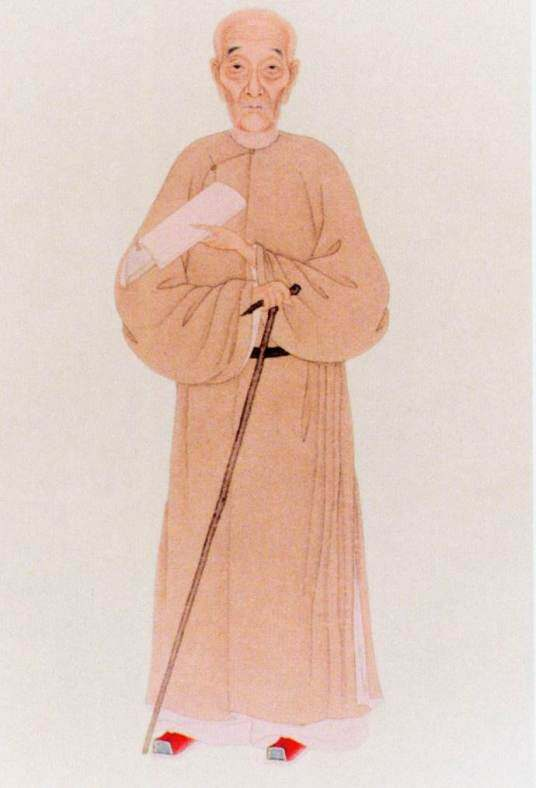
\includegraphics[height=2.65cm,keepaspectratio]{王念孙.jpg}\\
            \scriptsize 王念孙（1744--1832）

            \column{0.49\linewidth}
            \centering
            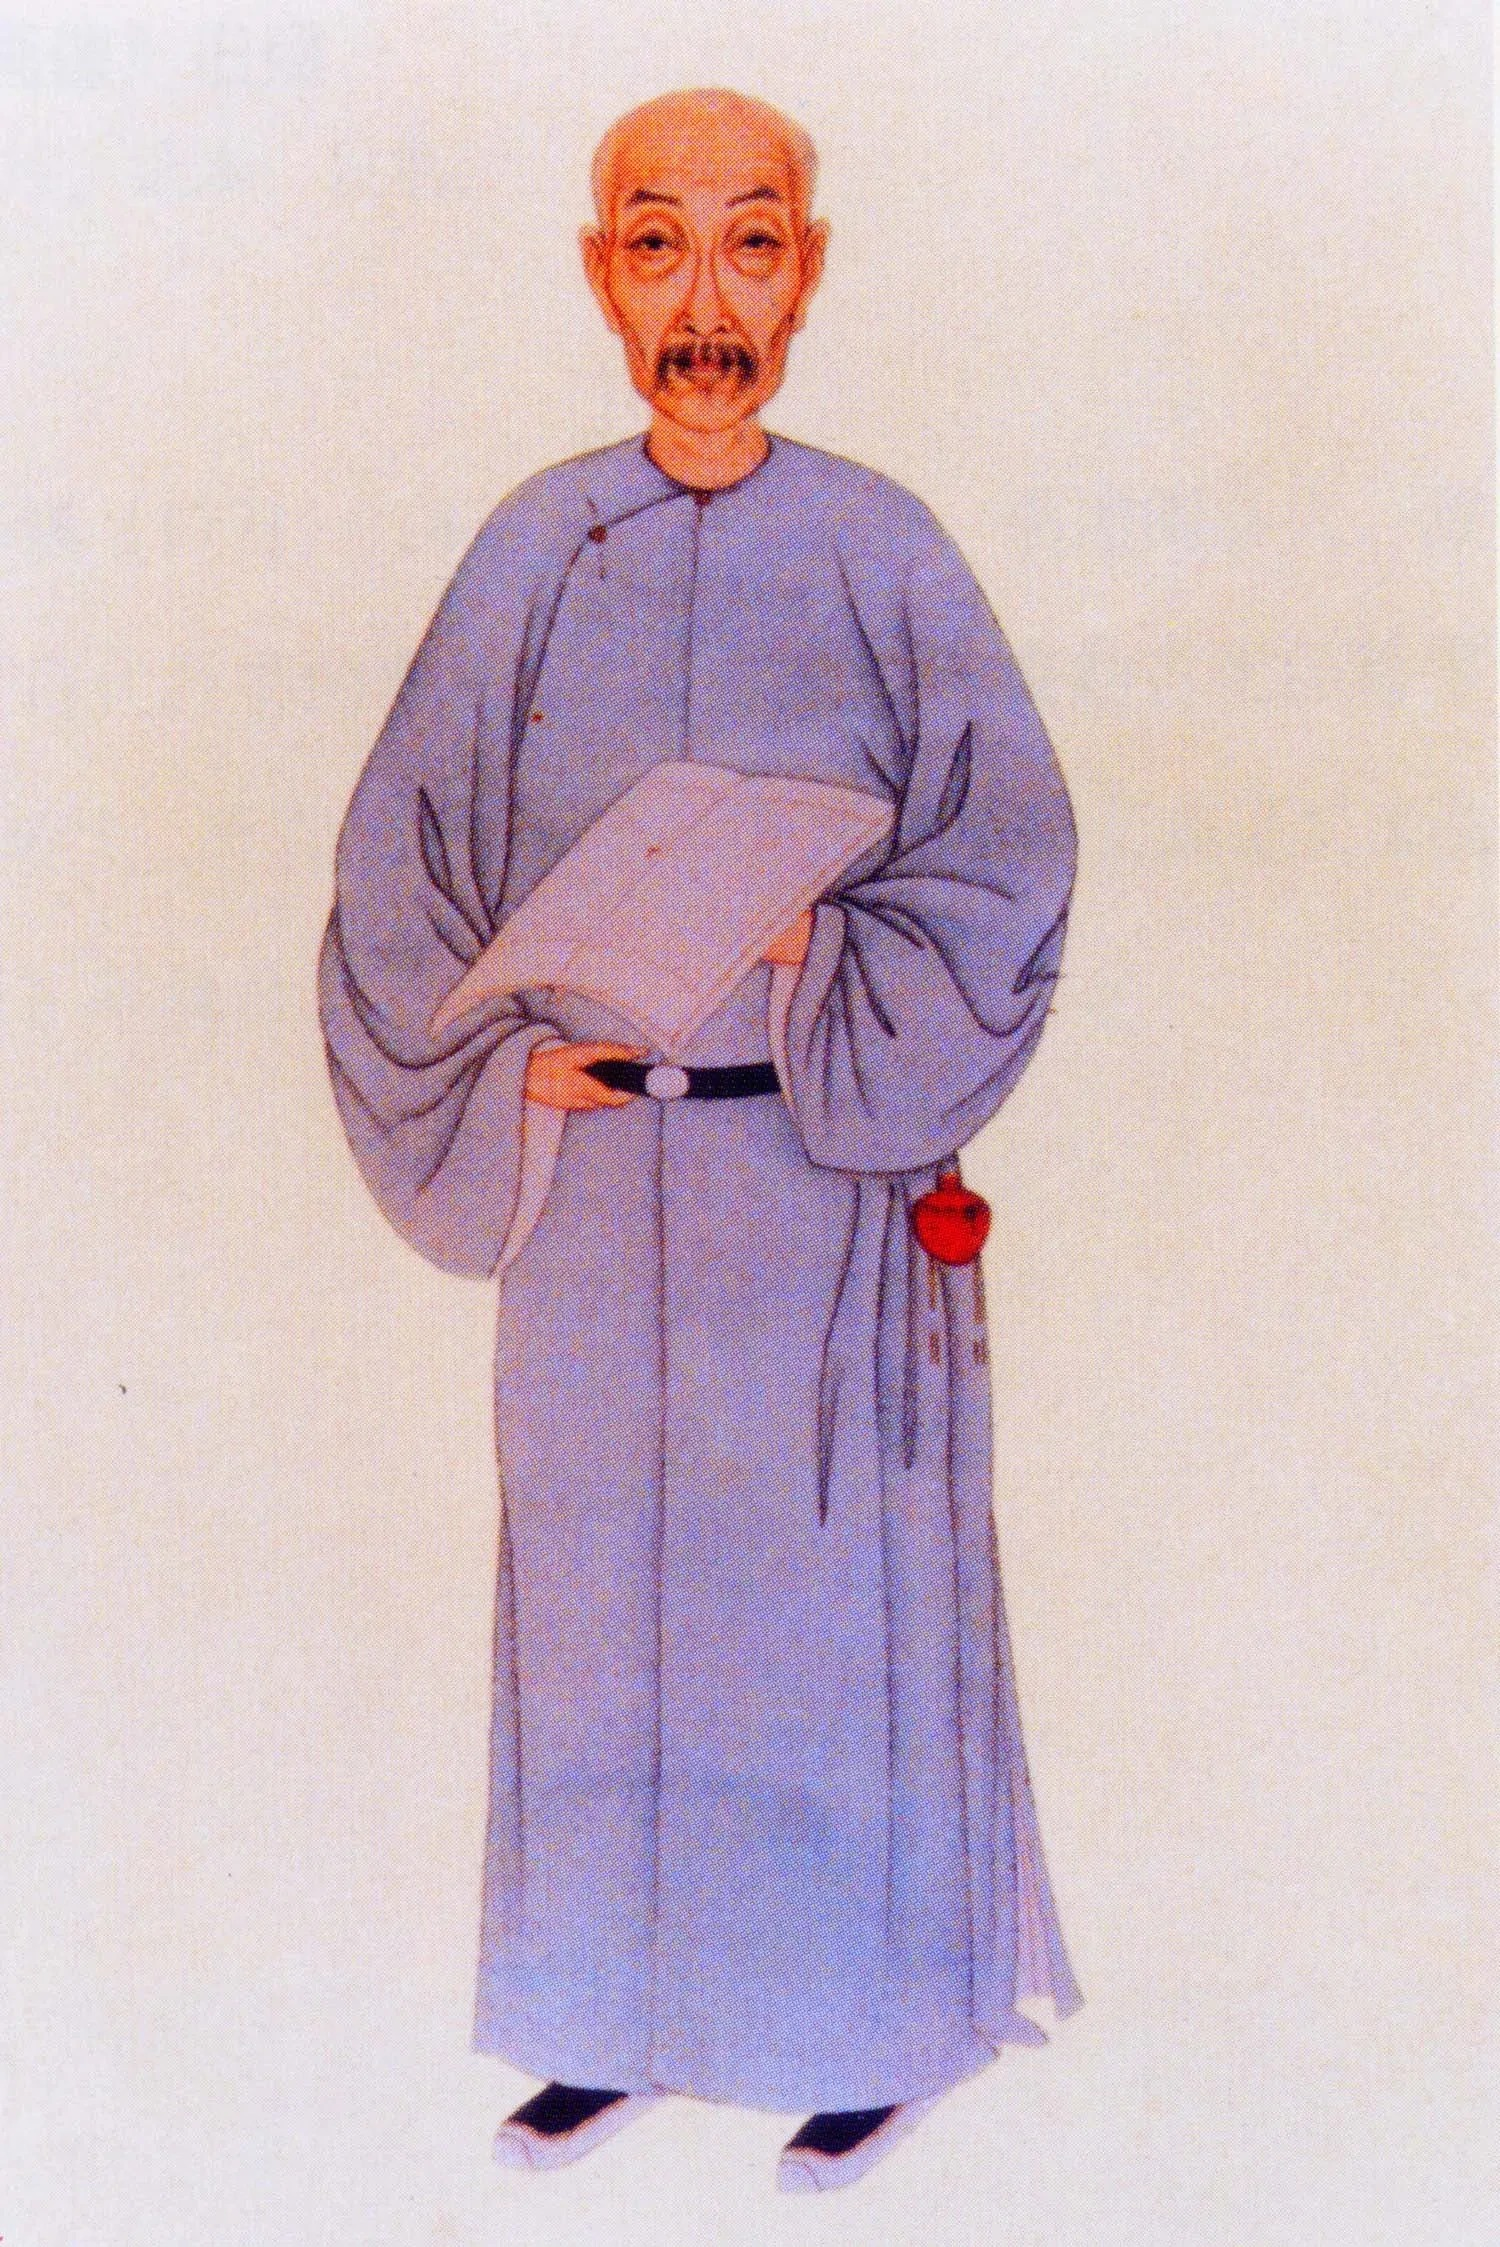
\includegraphics[height=2.65cm,keepaspectratio]{王引之.jpg}\\
            \scriptsize 王引之（1766--1834）
        \end{columns}

        % 右侧：王氏四种
        \column{0.53\textwidth}
        \vspace{0.35cm}

        \centering
        \key{王氏四种}\\[-1mm]
        {\scriptsize 本项目的核心材料边界}\par

        \vspace{0.10cm}

        \setlength{\tabcolsep}{0.10cm}
        \renewcommand{\arraystretch}{1.2}
        \begin{tabular}{c@{\hspace{0.08cm}}c@{\hspace{0.55cm}}c@{\hspace{0.08cm}}c}
            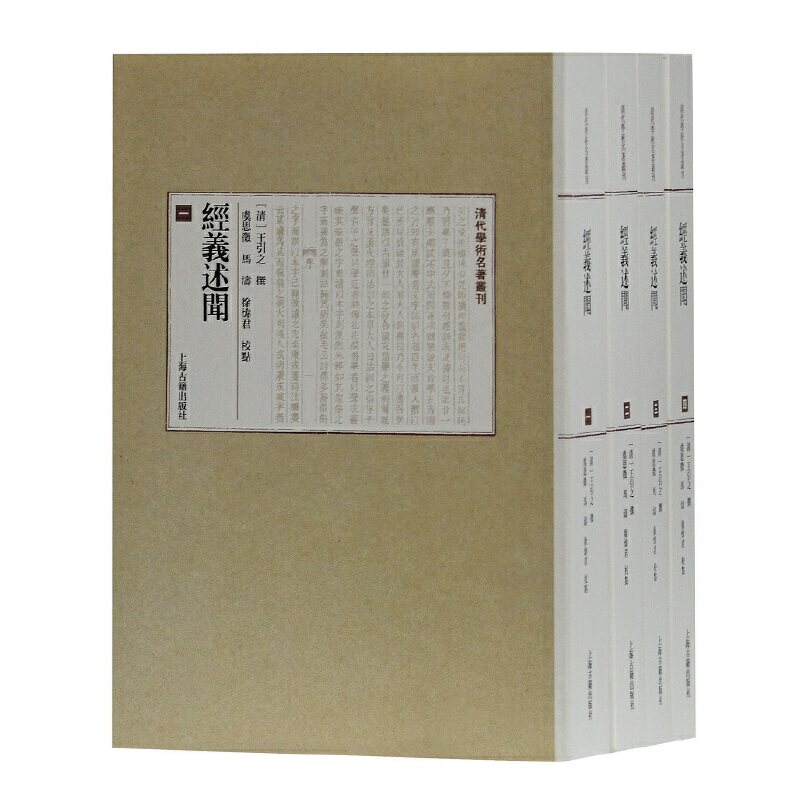
\includegraphics[height=2.60cm,keepaspectratio]{经义述闻.jpg}
            &
            \raisebox{0.50cm}{\scriptsize\shortstack{经\\义\\述\\闻}}
            &
            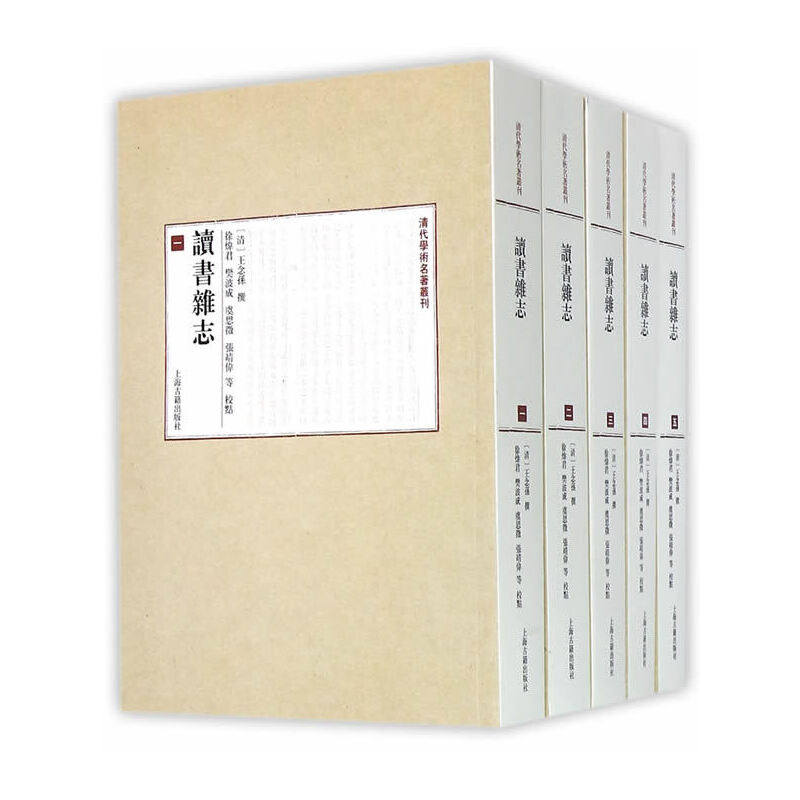
\includegraphics[height=2.60cm,keepaspectratio]{读书杂志.jpg}
            &
            \raisebox{0.50cm}{\scriptsize\shortstack{读\\书\\杂\\志}}
            \\[0.24cm]

            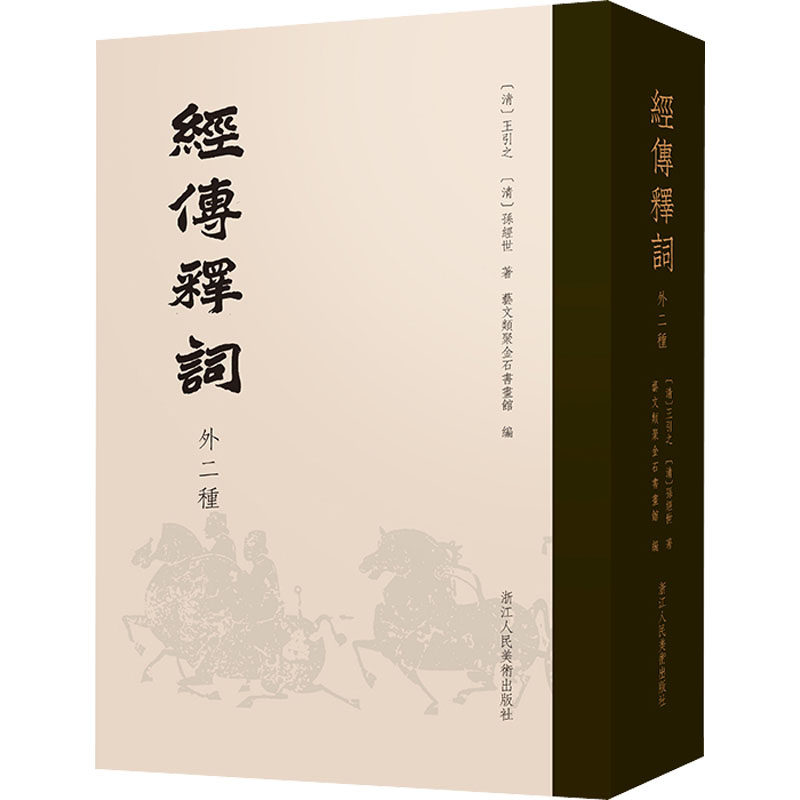
\includegraphics[height=2.60cm,keepaspectratio]{经传释词.jpg}
            &
            \raisebox{0.50cm}{\scriptsize\shortstack{经\\传\\释\\词}}
            &
            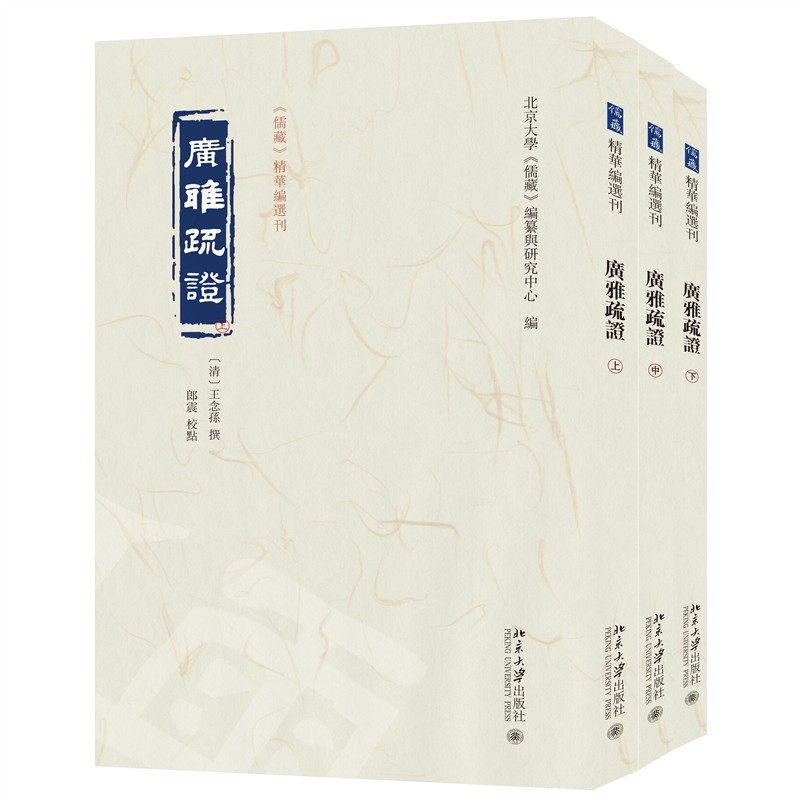
\includegraphics[height=2.60cm,keepaspectratio]{广雅疏证.jpg}
            &
            \raisebox{0.50cm}{\scriptsize\shortstack{广\\雅\\疏\\证}}
        \end{tabular}

    \end{columns}
\end{frame}

% PDF P4
\begin{frame}{立项依据与切入点}
    \small
    \begin{columns}[T]
        \column{0.48\textwidth}
        \begin{block}{研究对象明确}
            \begin{itemize}
                \item 范围明确：核心材料集中在王氏四种。
                \item 方法稳定：异文、校读、辞例、语境、因声求义等方法反复出现。
                \item 可结构化：材料核对、证据组织和判断步骤，可转为可保存、可检索、可复核的结构。
            \end{itemize}
        \end{block}
        \column{0.48\textwidth}
        \begin{block}{切入点独特}
            \begin{itemize}
                \item 现有平台侧重影像浏览、全文检索、条目定位，解决“材料在哪里”的问题。
                \item 但它更偏向简单的文本入口，难以呈现考据过程。
                \item 我们关注一条考据怎样成立，证据如何组织，并记录过程性方法知识。
            \end{itemize}
        \end{block}
    \end{columns}
    \vspace{0.18cm}
    \begin{center}
        \key{从“材料在哪里”推进到“一条考据怎样成立”}
    \end{center}
\end{frame}

% PDF P7：章节页
\section{研究方案}

% PDF P8
\begin{frame}{考据结构流程图}
    \begin{center}
        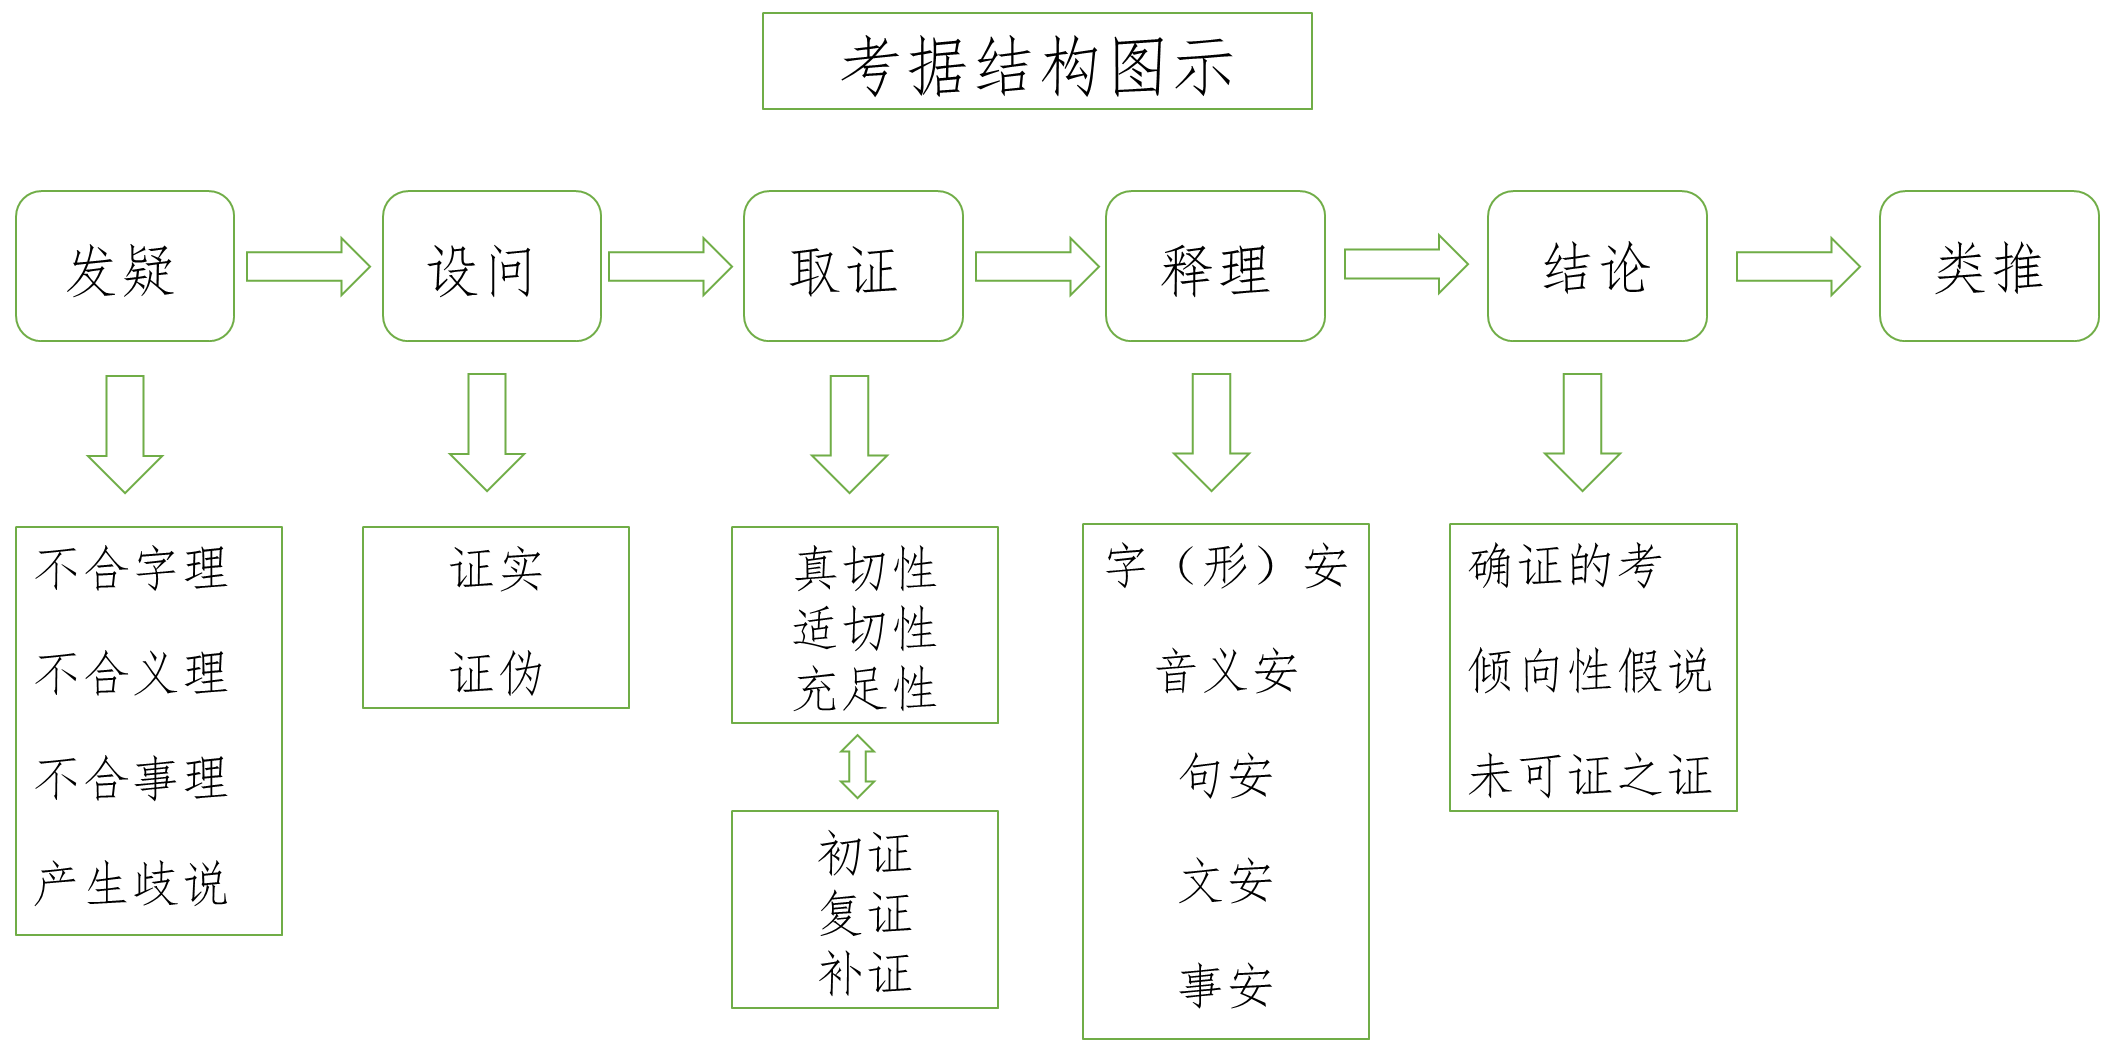
\includegraphics[height=0.68\textheight]{step.png}
    \end{center}
    \vspace{-0.05cm}
    \begin{center}
        \hint{据王宁《训诂学原理（增补本）》第 248 页整理，用于说明考据过程的基本环节。}
    \end{center}
\end{frame}

% PDF P9
\begin{frame}{代表案例：“造舟于河”}
    \small
    \begin{block}{《经义述闻·左传下》}
        《正义》承认“造舟为梁”是\key{比舟以为桥}，却又转训“造”为“至”；二王重新追问：“造”究竟应训为\key{比次}，还是训为\key{至}？
    \end{block}

    \vspace{0.15cm}

    {
    \renewcommand{\arraystretch}{1.20}
    \begin{tabularx}{\textwidth}{>{\bfseries\arraybackslash}p{0.08\textwidth} X}
        发疑 & 李巡、孙炎以“比”释“造舟”，孔颖达转训“造”为“至”，形成歧说。\\
        设问 & 王氏所要确认的是：“造”在此是否本有“比次”义。\\
        取证 & 以“造之言曹”“造、次一声之转”为音义证据；并举“薳氏之造”“属车之造”等书证。\\
        释理 & 以声求义，并用“副倅”“属车”“造舟”诸例互证，使字义、句义、文意相安。\\
        结论 & 李巡、孙炎所说“比舟”正切“造”义；转训为“至”“作”“诣”“成”皆属望文生训。\\
        类推 & 此例争点明确、证据层次清楚，适合展示“考据过程如何被结构化”。\\
    \end{tabularx}
    }
\end{frame}

% PDF P12
\begin{frame}{从考据过程到数据类型}
    \begin{center}
        \small\textbf{五种基本数据类型}
    \end{center}
    \vspace{-0.18cm}
    \begin{table}[h]
        \centering
        \small
        \begin{tabularx}{\textwidth}{>{\bfseries}l X X}
            \toprule
            类型 & 保存内容 & 展示作用 \\
            \midrule
            著作 & 二王著作、经典、工具书来源 & 保证出处可追溯 \\
            条目 & 原文、引文、二王论述片段 & 支持后续精细定位 \\
            案例 & 类型、构成、方法、结论、状态 & 保存考据主体 \\
            证据 & 书证、声训、义证、异文等 & 支撑复核与比较 \\
            词目 & 字、词、术语 & 提供检索入口 \\
            \bottomrule
        \end{tabularx}
    \end{table}
    \begin{center}
        \key{词目是入口，案例是中心，证据和出处保证可复核}
    \end{center}
\end{frame}

% PDF P10
\begin{frame}{训诂学内容入库}
    \begin{center}
        \small\textbf{训诂术语的层级落点}
    \end{center}
    \vspace{-0.24cm}
    \begin{table}[h]
        \centering
        \small
        \begin{tabularx}{0.96\textwidth}{>{\bfseries}p{0.15\textwidth} p{0.25\textwidth} X}
            \toprule
            层级 & 术语 & 系统中的落点 \\
            \midrule
            训释对象 & 文意训释 / 词义训释 & 区分句意判断与字词训释，避免把语境解释误作稳定义项 \\
            具体方法 & 形训、声训、义训 & 进入方法标签、释理说明和证据类型 \\
            声音路径 & 因声求义、通假 & 处理音近、字通与异文问题，形成核对事项 \\
            互证原则 & 形音义互求 & 作为同类案例比较和证据互证的观察框架 \\
            误释风险 & 望文生训 & 用于旧说裁断、反证说明和人工复核提醒 \\
            \bottomrule
        \end{tabularx}
    \end{table}
\end{frame}

% PDF P14
\begin{frame}{两条数据库搭建路线}
    \begin{columns}[T]
        \column{0.49\textwidth}
            \begin{exampleblock}{主数据库}
                \begin{itemize}
                    \item 保存较成熟的词目、案例、证据和出处。
                    \item 面向网站检索、案例详情页和统计展示。
                    \item 由整理后的结构化数据导出为网站快照。
                \end{itemize}
                \vspace{0.12cm}
                \centering
                {\scriptsize source.txt / dictionary.db / sqlite-snapshot.json}
            \end{exampleblock}
        \column{0.49\textwidth}
            \begin{exampleblock}{人工标注库}
                \begin{itemize}
                    \item 保存工作稿、AI 草案和人工复核材料。
                    \item 面向标注检查、证据补充和规则迭代。
                    \item 成熟后再进入主数据库。
                \end{itemize}
                \vspace{0.12cm}
                \centering
                {\scriptsize DOCX / annotations.db / annotation-snapshot.json}
            \end{exampleblock}
    \end{columns}
    \vspace{0.25cm}
    \begin{center}
        \key{成熟成果与研究工作稿分离；人工标注—AI草案—人工复核—规则迭代形成闭环}
    \end{center}
\end{frame}

% PDF P15
\begin{frame}{网站页面：多种材料形态共同展示}
    \begin{columns}[T]
        \column{0.50\textwidth}
        \begin{itemize}
            \item 首页：用“造舟于河”讲清一条考据。
            \item 数据库页：字词、案例、书证、结构四种视角，串联不同考据。
            \item 详情页：展开证据链和出处。
            \item 术语页：辅助理解训诂概念。
            \item 人工标注库：展示 DOCX 标注转出的结构化成果。
            \item AI 释证：输出草案，同时展开引用材料。
        \end{itemize}
        \column{0.50\textwidth}
        \vspace{-0.2cm}
        \centering
        \hspace{0.3cm}
            {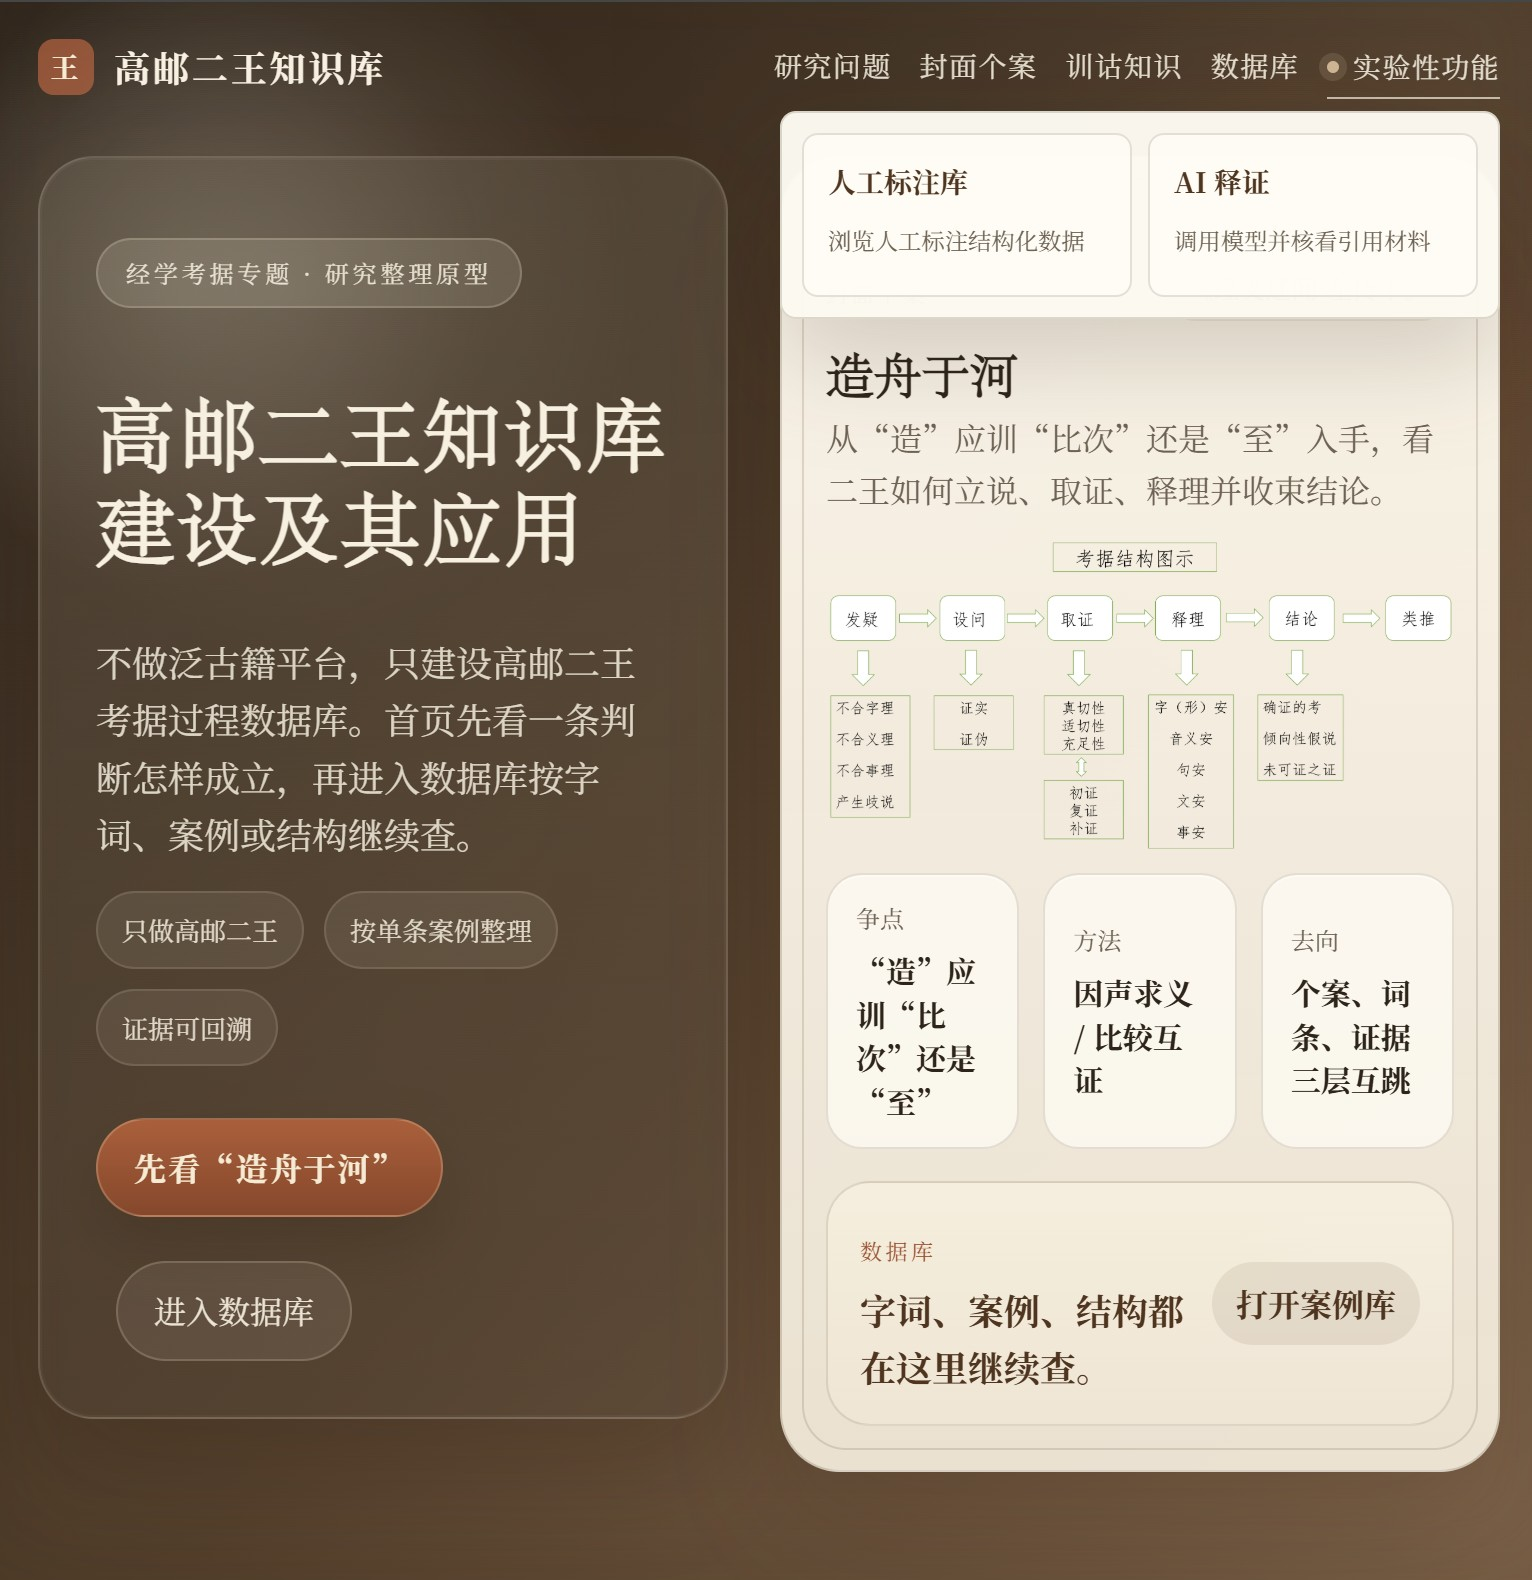
\includegraphics[width=0.96\linewidth,height=0.74\textheight,keepaspectratio]{homepage.jpg}}
    \end{columns}
    \vspace{0.1cm}
    \begin{center}
        \small \url{https://gaoyou-demo1.up.railway.app/}
    \end{center}
\end{frame}

% PDF P16：章节页
\section{研究创新}

% PDF P17
\begin{frame}{古典人文学术与现代数智技术的融合}
    \begin{columns}[T]
        \column{0.31\textwidth}
        \begin{exampleblock}{古典人文学术}
            文献细读、出处核验、训诂判断、效度辨析。
        \end{exampleblock}
        \column{0.31\textwidth}
        \begin{exampleblock}{数据组织}
            词目、案例、证据、出处、过程步骤的组织与展示。
        \end{exampleblock}
        \column{0.31\textwidth}
        \begin{exampleblock}{智能辅助}
            人工库相关案例检索、AI 释证草案、引用展开核对。
        \end{exampleblock}
    \end{columns}
    \vspace{0.40cm}
    \begin{block}{如何融合？}
        使校勘学、训诂学等古典人文学术，作为数据建模和人工复核的规则；\\
        使数据库与 AI 等现代数智技术，让人文研究过程可展示、可复核、可扩展。
    \end{block}
\end{frame}

% PDF P18
\begin{frame}{泛化能力：从材料到平台}
    \begin{block}{方法迁移}
        迁移我们的整理流程：把原文、引文和论述转成可复核的结构，再由界面支持检索、阅读和教学。
    \end{block}
    \begin{columns}[T]
        \column{0.50\textwidth}
        \begin{exampleblock}{泛化机制}
            \begin{itemize}
                \item 文本：原典、引文、学者论述
                \item 结构：字段、证据类型、过程步骤
                \item 界面：检索、详情页、引用展开
            \end{itemize}
        \end{exampleblock}
        \column{0.50\textwidth}
        \begin{exampleblock}{迁移方向}
            \begin{itemize}
                \item 材料：经典注疏争议、出土文献、小学专书
                \item 平台：考据笔记整理、课堂阅读训练
                \item 目标：让同类问题可比较、可复核
            \end{itemize}
        \end{exampleblock}
    \end{columns}
    \vspace{0.25cm}
    \begin{center}
        \pill{文本结构化} \quad \pill{过程可复核} \quad \pill{场景可迁移}
    \end{center}
\end{frame}

% PDF P19
\begin{frame}{AI 在项目中的运用}
    \begin{columns}[T]
        \column{0.48\textwidth}
        \begin{block}{可以辅助}
            \begin{itemize}
                \item 相似案例检索
                \item 证据片段匹配
                \item 结构化草稿生成
                \item 提醒人工复核点
            \end{itemize}
        \end{block}
        \column{0.48\textwidth}
        \begin{block}{不能替代}
            \begin{itemize}
                \item 原文与版本核对
                \item 通假方向判断
                \item 词义与文意区分
                \item 最终学术结论确定
            \end{itemize}
        \end{block}
    \end{columns}
\end{frame}

% PDF P20：章节页
\section{项目规划和预期成果}

% PDF P21
\begin{frame}{当前数据基础}
    \vspace{0.25cm}
    \begin{center}
        \numstat{49}{著作来源}
        \numstat{3385}{词目}
        \numstat{815}{案例}
        \numstat{7120}{证据}
    \end{center}
    \vspace{0.6cm}
    \begin{block}{人工标注灰度库}
        当前另有 3 个标注文档、17 条案例、44 个词目、121 条证据、64 个过程步骤。\\
        主库先完成词目、案例、证据闭环，条目层后续补实；\\
        标注库保存工作稿、AI 整理与人工复核材料。
    \end{block}
\end{frame}

% PDF P22
\begin{frame}{阶段计划与预期成果}
    \small
    \begin{table}[h]
        \centering
        \setlength{\tabcolsep}{4pt}
        \renewcommand{\arraystretch}{1.08}
        \begin{tabularx}{\textwidth}{>{\bfseries}l X X}
            \toprule
            阶段 & 推进重点 & 交付成果 \\
            \midrule
            A & 统一底本、出处、案例模板和术语口径 & 字段规范、首批案例清单 \\
            B & 建立词目、案例、证据的检索闭环 & 可视化、可检索的数据平台 \\
            C & 扩充精选案例，完善典型疑难处理路径 & 不少于 300 条精选案例；考据教学文件 \\
            D & 探索项目方法向其他考据主题迁移 & 泛化应用说明；人机协作标注流程 \\
            \bottomrule
        \end{tabularx}
    \end{table}
    \begin{block}{最终形成}
        《高邮二王考据案例标注规范》、可复用数据库路线、典型疑难处理路径整理说明，以及《高邮二王考据研究》读书报告或研究论文。
    \end{block}
\end{frame}

% PDF P22
\begin{frame}[plain]
    \vspace{0.95cm}
    \begin{center}
        \begin{beamercolorbox}[wd=0.72\textwidth,sep=0.55cm,center,rounded=true,shadow=true]{block body}
            {\Huge\textcolor{rucRed}{\textbf{谢谢老师}}}\\[0.38cm]
            {\Large 恳请各位老师批评指正}\\[0.36cm]
            \textcolor{rucRed}{\rule{0.42\linewidth}{0.6pt}}\\[0.28cm]
            {\small 高邮二王考据过程知识库构建及应用}
        \end{beamercolorbox}
    \end{center}
\end{frame}

\end{document}
